
\documentclass[a4paper, 10pt]{article}  

\usepackage{geometry}
\geometry{a4paper, margin=1in}
    
    
\usepackage{verbatim}
\usepackage{graphicx}
\usepackage{pdfpages}
\usepackage{cite}
\usepackage{listings}
\usepackage{float}

\lstset{
	tabsize=2,
	breaklines=true
}

\setlength{\parskip}{1em}

\title{\LARGE \bf Beckhoff Progress Report 1\\Engineering Practice 6: Design 228 711}
\author{Marc Alexander Sferrazza (Alex) 12164165 | Abeer Ali Syed (Abeer) 12237898 \\ Divraj Singh (Div) 14076417 | Maen Algharibeh (Maen) 10256119
\thanks{This work was not supported by any organization}
\thanks{Faculty of Mechatronics Engineering, Massey University, Albany, Auckland, New Zealand
        {\tt\small Progress of project: https://github.com/alex1v1a/Beckhoff-PLC-Project-2017} } }

\begin{document}

\maketitle

\begin{figure}[H]
  
\includegraphics[width=\linewidth]{images/beckhoff}
  \label{fig:opencv}
\end{figure}

\thispagestyle{empty}
\pagestyle{plain}


%%%%%%%%%%%%%%%%%%%%%%%%%%%%%%%%%%%%%%%%%%%%%%%%%%%%%%%%%%%%%%%%%%%%%%%%%%%%%%%%

\begin{abstract}
This report includes the project plan that indicates key elements of the project and also highlights some key decisions. The report also provides basic technical principles and their relevance to this project. Moreover, some creative elements have been added in multiple areas of this project. 

The aim of this project is to create a system that reads data from a sensor using the Beckhoff industrial PC remotely via a cloud storage and reports the data to a mobile application for wireless operation monitoring and management. The mobile application will prompt the user with a message if a sensor exceeds a certain limit and allows authorisation and complete control of the system to proceed or cancel the operation depending on the user's? need.
\end{abstract}

\clearpage
\tableofcontents
\thispagestyle{empty}
\clearpage

%%%%%%%%%%%%%%%%%%%%%%%%%%%%%%%%%%%%%%%%%%%%%%%%%%%%%%%%%%%%%%%%%%%%%%%%%%%%%%%%
%%%%%%%%%%%%%%%%%%%%%%%%%%%%%%%%%%%%%%%%%%%%%%%%%%%%%%%%%%%%%%%%%%%%%%%%%%%%%%%%

\setcounter{page}{1}

\section{Project Context}

The main objective of this project was to create a system using the Beckhoff industrial PC, which allows a user to read data from a particular sensor wirelessly through a cloud storage.

Additionally, deliver alternative reactions to advance the tasks with a seamless integration of automation. Using the twin-CAT environment and the EtherCAT protocol with the Beckhoff PLC system, will allow a universally compatible sensor module that will provide a real-time status on a mobile device application. This will also prompt the user with continuous updates to manage the situation remotely instead of constant manual intervention.

A more specific approach is required for particular situation, the system will have a �universal fit to industrial sensors and provide modified solutions for different clients? needs.

%%%%%%%%%%%%%%%%%%%%%%%%%%%%%%%%%%%%%%%%%%%%%%%%%%%%%%%%%%%%%%%%%%%%%%%%%%%%%%%%

\section{Project Planning and Management}

We choose to use a proximity detector which gives a voltage output; how can we change this to milliamp signal for Beckhoff input? (4-20mA Beckhoff readable range)

\begin{itemize}
\item Reduced overall running costs on the production line decreasing costs of production More efficient and time managed system
\item Reduced time spent on troubleshooting and maintaining control systems
\item Wireless anytime access to the production process allowing maintenance and actions to be carried out without having someone physically drive out on site
\item Increase in demand of Beckhoff products due to the rise of mobile based application
\end{itemize}

Less running costs due to issues being solved through the mobile application leading to a decrease in carbon emissions and costs of production Any change proposed to the current plan must go through an authorisation process in which a team meeting will take place. All aspects and consequences must be discussed. A vote will be carried out to resolve the change. Incase of a split decision, Dr. Frazer Noble, Dr. Khalid Arif (mentors/supervisors) and Omer Naveed (Beckhoff representative) will be consulted to each of the desired goals. The project consent is not applicable to change. Also other content of this project charter which is not subject to change must be agreed upon by all the team members at the launch of this project.


%\begin{figure}[H]
%  \includegraphics[width=\linewidth]{images/}
%  \caption{}
%  \label{fig:}
%\end{figure}


%%%%%%%%%%%%%%%%%%%%%%%%%%%%%%%%%%%%%%%%%%%%%%%%%%%%%%%%%%%%%%%%%%%%%%%%%%%%%%%%

\section{Engineering Problem Solving}

\begin{itemize}
\item How it works??\item Is it common practice in industry? Yes, why??\item What is it going to output??\item How is this used in industry practice??\item What equipment is required? (The modules we already have, components email)?\item What does it need to generate??\end{itemize}

\clearpage
Program the Beckhoff PC to take in the sensor output from the signal converter PCB and output a text file. A folder will be created to house many files which are: 
\begin{itemize}
\item First file will be programmed to display live output of the sensor max of 1000 lines which are recorded entries?\item A Write file containing an error list from PC read by the app and assign an ID to each error for example: ?ERROR 01: Sensor stopped? ?\item The third file will read the file in the PC from the mobile app and output the solution matched to the error for example: ?Restart the system?.?\item The fourth file housed in the folder will act as a data logger which will contain recorded sensor entries for the past 100,000 entries.?\end{itemize}

This project's scope covers solutions related to troubleshooting faults on a production process without being present at the plant. Since we live in an era where most individuals carry smart phones we have decided to take advantage of this concept and implement a mobile application.


This mobile application will allow the user to take the troubleshooting steps necessary to eliminate an error. This troubleshooting step could be as simple as turning on a fan when a temperature sensor reads a critical value. For example, the temperature inside a factory may be above the accepted value, this would cause the mobile app to display an error message and ask the user if he wishes to turn on the power source connected to a fan which would bring the temperature in the factory to an appropriate level.

This app will be written in swift using XCode. At this stage, we currently have an app template with one button and a title which reads ?Beckhoff App V1?. At first, the application will only be available for IOS devices however this may change in the upcoming weeks.

\begin{figure}[H]
  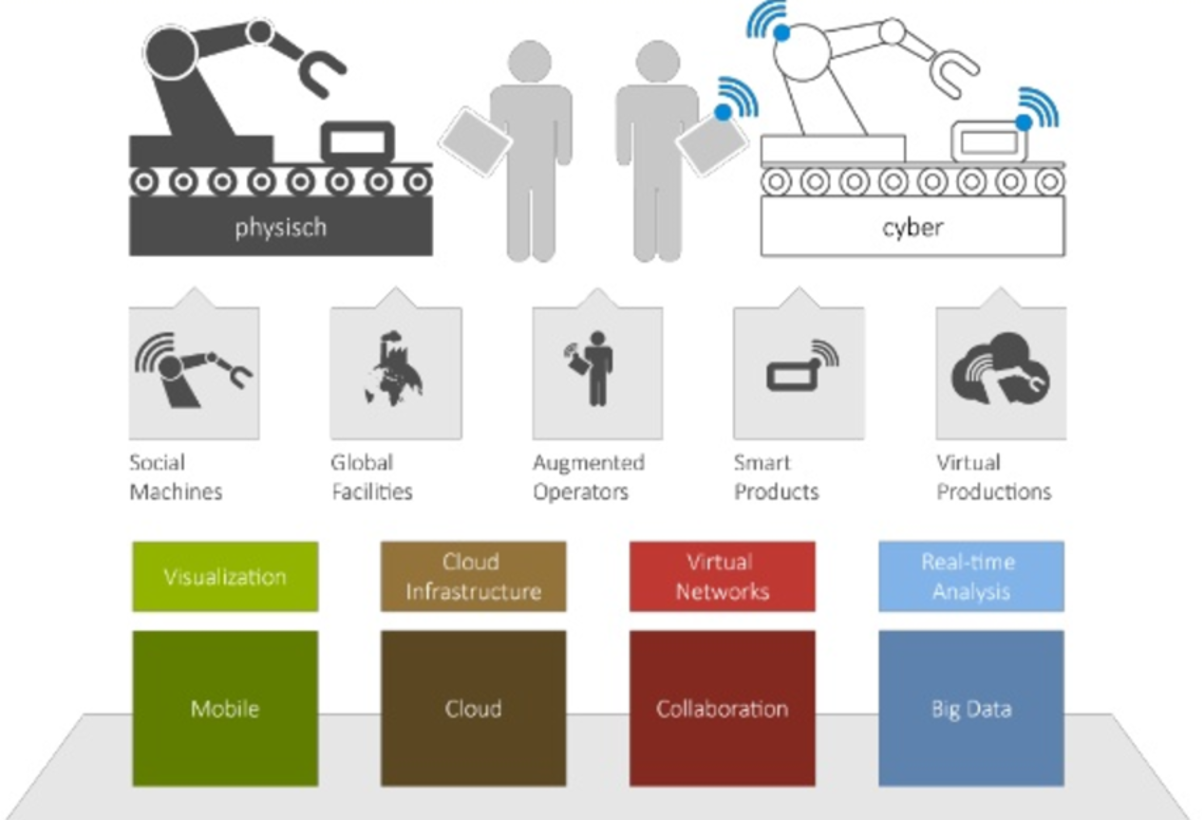
\includegraphics[width=\linewidth]{images/process}
  \caption{Breakdown of smart manufacturing}
  \label{fig:Breakdown of smart manufacturing}
  \end{figure}

To establish a secure and safe electrical connection between the sensor and the Beckhoff system, the industry standard for electrical connection must be met. The Beckhoff systems provide two technologies to connect wiring on their modules (i.e. Standard and Pluggable wiring). The Standard wiring uses a screw-less and spring-loaded technology which allows for a fast and simple assembly. 

The Pluggable wiring uses a technology which allows for all wires to be plugged off and be replaced with a different set of wires quickly. The technology used in this project will depend on the sensor used. The module used for digital input is the EK1814 and it used Standard wiring technology, while the EL3058 provides analog input terminals and uses the Pluggable wiring technology. An advantage for both these technology is that they do not require special wiring plugs to establish an electric connection and wires can be securely plugged into the modules via the spring-loaded technology. 


PCB 0-5V to 4-20mA converter (SEE BELOW)
Inside the PLC an analog to digital converter transforms the signal received, this value can be negative. The signal ranges with a minimum input of 4mA to maximum of 20mA; this range is sourced from the voltage through a given resistance and is used commonly in standard PLC 24VDC practice. This configuration is know as Current looping, and when the input is below 4mA a receiver may be able to recognise this as the negative values.

Not only is the option of measuring current over voltage simpler and easier to configure, there is less wire needed and the signals? quality is not lost over long distances, as like when voltage degrades over a long distance. Current loops also use less power and are less prone to interference than a voltage signal. 

While current loops are a cost effective solution in may applications, they are unable to transmit more than one specific signal. By adding more loops to a system there could potentially be issues from induction influence on ground loops; therefore it is necessary to properly isolate the convoluting loops.

Taking the input from a analog proximity sensor would require a current conversion feed into the the loop, which in turn is reviewed and 4-20mA signal interpreted to a scaled output, eg a 10 bit signal from 0-1024 producing a translation from 0-16 pound or 1 bar rate.

\begin{figure}[H]
  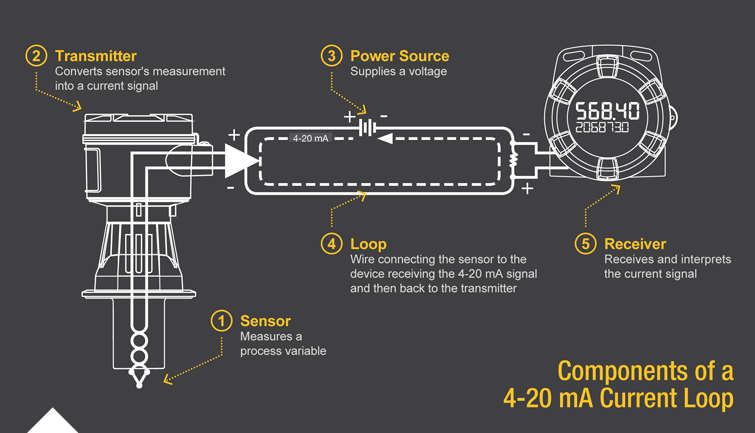
\includegraphics[width=\linewidth]{images/currentloop}
  \caption{Example of a current loop circuit}
  \label{fig:Example of a current loop circuit}
\end{figure}

The use of current loops are widely used as they are cost effective in smaller scenarios and provide higher accuracy over that of a voltage measurement. 

%http://control.com/thread/1026235722
%https://www.predig.com/indicatorpage/back-basics-fundamentals-4-20-ma-current-loops
%http://www.walchem.com/TechSupport/WebM/PDFs/4-20ma\%20Input\%20Wiring.pdf
%https://www.acromag.com/sites/default/files/Acromag_Intro_TwoWire_Transmitters_4_20mA_Current_Loop_904A.pdf



%%%%%%%%%%%%%%%%%%%%%%%%%%%%%%%%%%%%%%%%%%%%%%%%%%%%%%%%%%%%%%%%%%%%%%%%%%%%%%%%

\section{Creativity}

The current looping PCB that will be designed for the Beckhoff system will be able to read data from a variety of sensors (e.g. �proximity, temperature, barometer) and convert the signal between 4 to 20 mA. The PCB should be able to achieve this without losing any useful information (e.g. resolution or accuracy). Future development of the PCB should be able to read and output data from multiple sensors at once.

Networking, connecting the Beckhoff unit to a network and treating it as a server to host the output for the sensors, and using port forwarding with triggering to the unit to read from external networks. The app will connect to the public IP of the Beckhoff unit to access the output from a ported folder. The app will read live time and can be updated on request as long as there is a stable network connection.

%\begin{figure}[H]
%  \includegraphics[width=\linewidth]{images/}
%  \caption{}
%  \label{fig:}
%\end{figure}


%%%%%%%%%%%%%%%%%%%%%%%%%%%%%%%%%%%%%%%%%%%%%%%%%%%%%%%%%%%%%%%%%%%%%%%%%%%%%%%%

\section{Progress}
The development of the project has yet to come but is underway. The parts have just been received last week for the beckhoff unit so have yet to explore its features; but the initial design of the app has been developed ready for when the module has been setup.

\section{Conclusion}

In conclusion, the team aims to produce a solution that allows the user to efficiently and effectively communicate remotely with the Beckhoff PLCs via their mobile device. The team will achieve this task with the help of the project plan as it will provide us with a clear direction towards milestones and our final goal. 

The PCB design will allow the user to plug in a range of many different sensor and will convert the sensor?s voltage output to a current output to a limited range of 4 to 20mA of current. This PCB will work with the Beckhoff system and act as an intermediate step between the sensor and the programmable logic controller. 

%%%%%%%%%%%%%%%%%%%%%%%%%%%%%%%%%%%%%%%%%%%%%%%%%%%%%%%%%%%%%%%%%%%%%%%%%%%%%%%%
%%%%%%%%%%%%%%%%%%%%%%%%%%%%%%%%%%%%%%%%%%%%%%%%%%%%%%%%%%%%%%%%%%%%%%%%%%%%%%%%

\nocite{*}
\bibliographystyle{ieeetr}
\bibliography{references}

%%%%%%%%%%%%%%%%%%%%%%%%%%%%%%%%%%%%%%%%%%%%%%%%%%%%%%%%%%%%%%%%%%%%%%%%%%%%%%%%
%%%%%%%%%%%%%%%%%%%%%%%%%%%%%%%%%%%%%%%%%%%%%%%%%%%%%%%%%%%%%%%%%%%%%%%%%%%%%%%%

%\clearpage
\section*{APPENDIX}

\begin{lstlisting}[language = C++]
Attached source code for iOS app developed in XCODE

Please see Abeer for a copy

\end{lstlisting}

\end{document}
